
\section{\igh{} constant-region evolution in the Atherinomorpha}
\label{sec:locus_comparative}

The characterised \igh{} loci of \nfu, \xma and medaka together reveal a high degree of variability in structure and function across the Atherinomorpha, the parent clade of the Cyprinidontiformes (including \Nfu and \Xma) and the Beloniformes (including medaka). Several unusual features (including the loss of \igh{Z}, an inverted sublocus, and an unusual splicing pattern of \igh{M-TM}) are shared between medaka and turquoise killifish, but absent in platyfish (\Cref{fig:species-tree-small}), indicating either an independent origin in the former two species or a reversion to the primitive state in the latter. In addition, the copy number, exon usage and orientation of constant regions of other isotypes differs among the three species, raising the further question of how, when and why these changes occurred. 

In order to investigate a subset of these questions with a greater degree of phylogenetic resolution, \igh{} constant regions were identified and analysed in a further ten cyprinodontiform species (\Cref{fig:species-tree-large-taxa}, \Cref{tab:cyprinodontiform-genomes}), as well as in a new and improved genome assembly of medaka (Genbank accession GCA\_002234675.1), using the same methods described for \Nfu and \Xma (\Cref{sec:nfu-locus-constant,sec:nfu-locus-variable}). The exons so identified (\Cref{fig:ch-tree-all}) were then grouped by order, exon type and spatial proximity to identify contiguous constant-regions, enabling the presence/absence and number of constant regions of each isotype to be estimated for each species. % TODO: Link to methods chapter?
The results of this analysis (\Cref{fig:multispecies-ch-regions}, \Cref{tab:multispecies-ch-regions-1,tab:multispecies-ch-regions-2,tab:multispecies-ch-regions-3}) demonstrate that every species investigated possesses at least one complete \igh{M} and \igh{D} constant region in tandem, with several species exhibiting multiple such regions. Apart from \Nfu and medaka, only \textit{Nothobranchius orthonotus} was identified as clearly possessing adjacent constant regions in opposite orientation, indicating the presence of at least one sublocus in antisense; however, the fragmented nature of the \igh{} locus assembly in many analysed species prevented a confident exclusion of such loci in other cases.

% Constant regions were evaluated as ``complete" if they possessed all expected \ch exons and TM1 (TM2 was not included due to the extremely short length of its conserved coding sequence) and as ``pseudogenised" if at least one exon contained a detectable frameshift, nonsense mutation, or truncation; regions missing exons due to missing genomic sequence were not annotated as either complete or pseudogenised. % TODO: To methods

\begin{table}[bh!]
\centering
\begin{threeparttable}
\begin{tabular}{>{\itshape}l>{\itshape}llc}\toprule
\textnormal{\textbf{Genus}} & \textnormal{\textbf{Species}} & \textbf{Common Name} & \textbf{GenBank Assembly Accession}\\\midrule
Nothobranchius & furzeri & Turquoise killifish & NA\tnote{1}\\\midrule
Xiphophorus & maculatus & Southern platyfish & GCA\_002775205.2\\
Austrofundulus & limnaeus & -- & GCA\_001266775.1\\
Fundulus & heteroclitus & Mummichog & GCA\_000826765.1\\
Poecilia & formosa & Amazon molly & GCA\_000485575.1\\
Poecilia & reticulata & Guppy & GCA\_000633615.1\\
Cyprinodon & variegatus & Sheepshead minnow & GCA\_000732505.1\\
Kryptolebias & marmoratus & Mangrove rivulus & GCA\_001649575.1\\\midrule
Aphyosemion & australe & Lyretail panchax & NA\tnote{2}\\
Callopanchax & toddi & -- & NA\tnote{2}\\
Pachypanchax & playfairii & Golden panchax & NA\tnote{2}\\
Nothobranchius & orthonotus & Spotted killifish & NA\tnote{2}\\\midrule
Oryzias & latipes & Medaka & GCA\_002234675.1\\
\bottomrule\end{tabular}
\begin{tablenotes}
\item[1] Willemsen \textit{et al.}, unpublished at time of writing
\item[2] Cui \textit{et al.}, unpublished at time of writing
\end{tablenotes} % TODO: Update once publication info is available
\end{threeparttable}
\vspace{0.5em}
\caption{Genome assemblies used to identify putative \textit{IGH} locus sequences in cyprinodontiform fishes.}
\label{tab:cyprinodontiform-genomes}
\end{table}

\begin{figure}
\centering
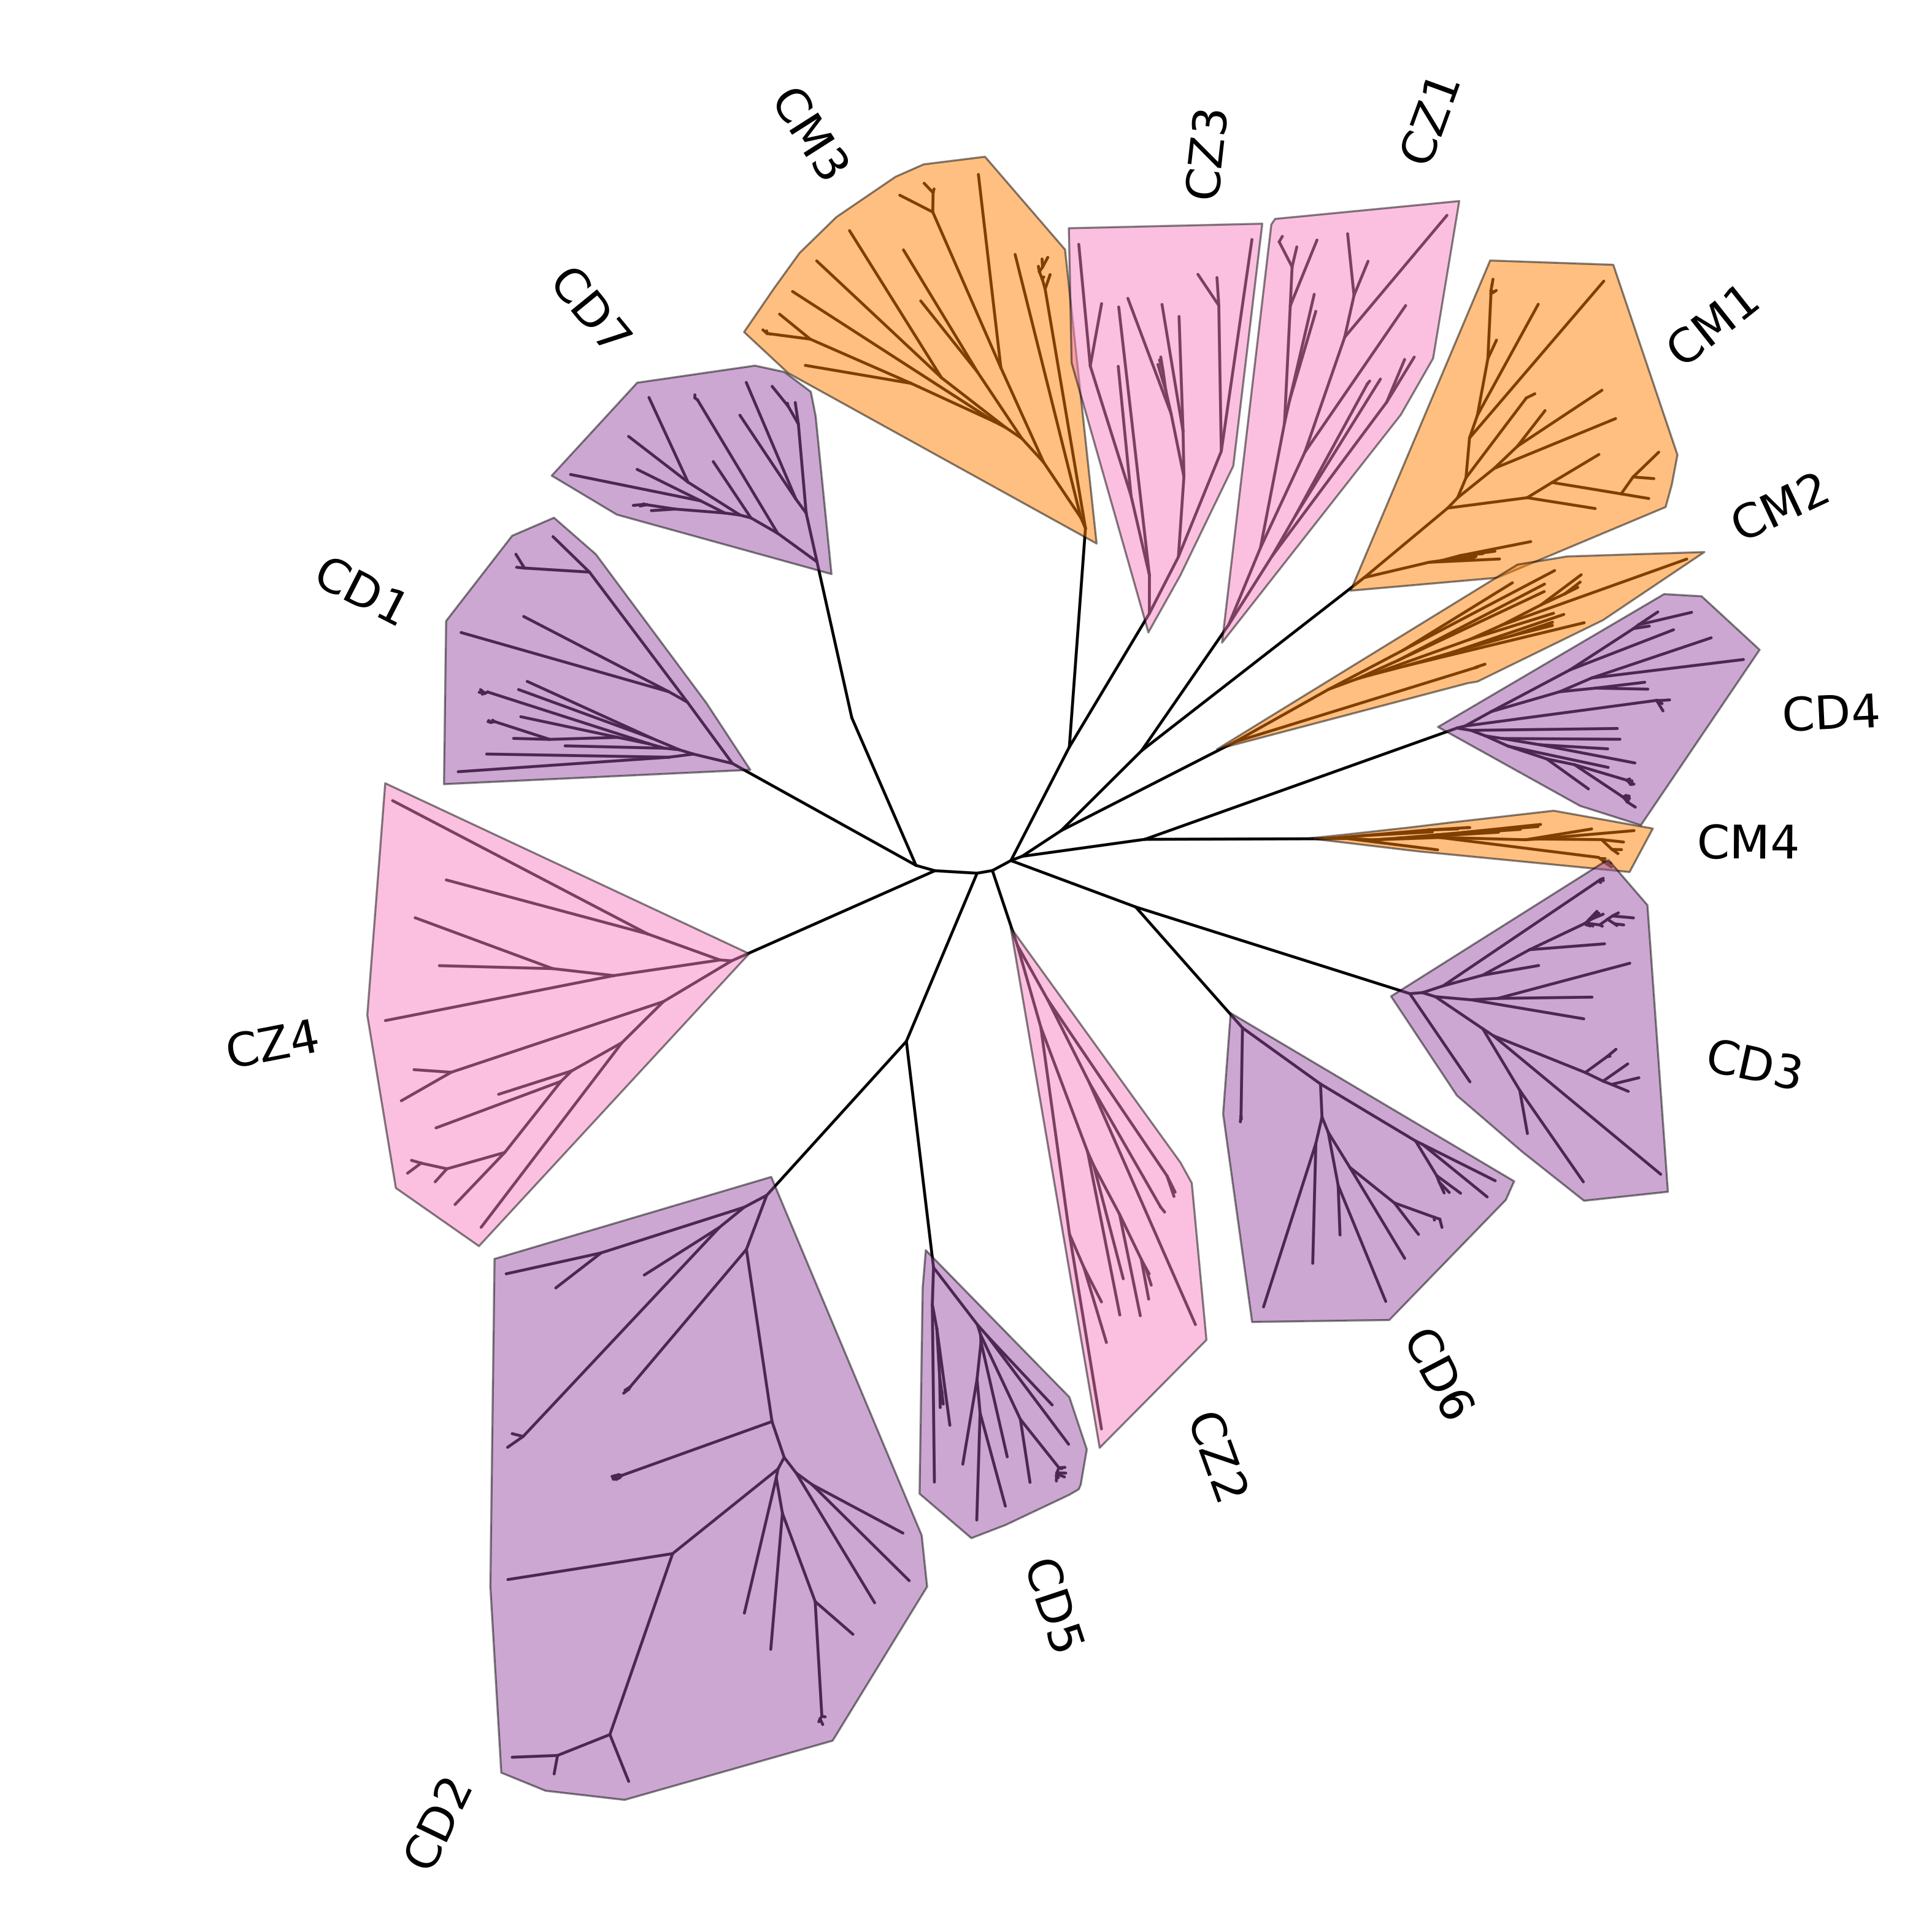
\includegraphics[width=0.9\textwidth]{_Figures/png/ch-tree-all}
\caption[\ch exons in the Atherinomorpha]{\textbf{\ch exons in the Atherinomorpha:} Unrooted phylogram of \ch exons in thirteen fish species from the Atherinomorpha, constructed using \program{PRANK} and \program{RAxML}. Each exon type is clustered separately in the tree topology, indicating that the types of the identified exons have all been correctly annotated.}
\label{fig:ch-tree-all}
\end{figure}

\begin{figure}
\centering
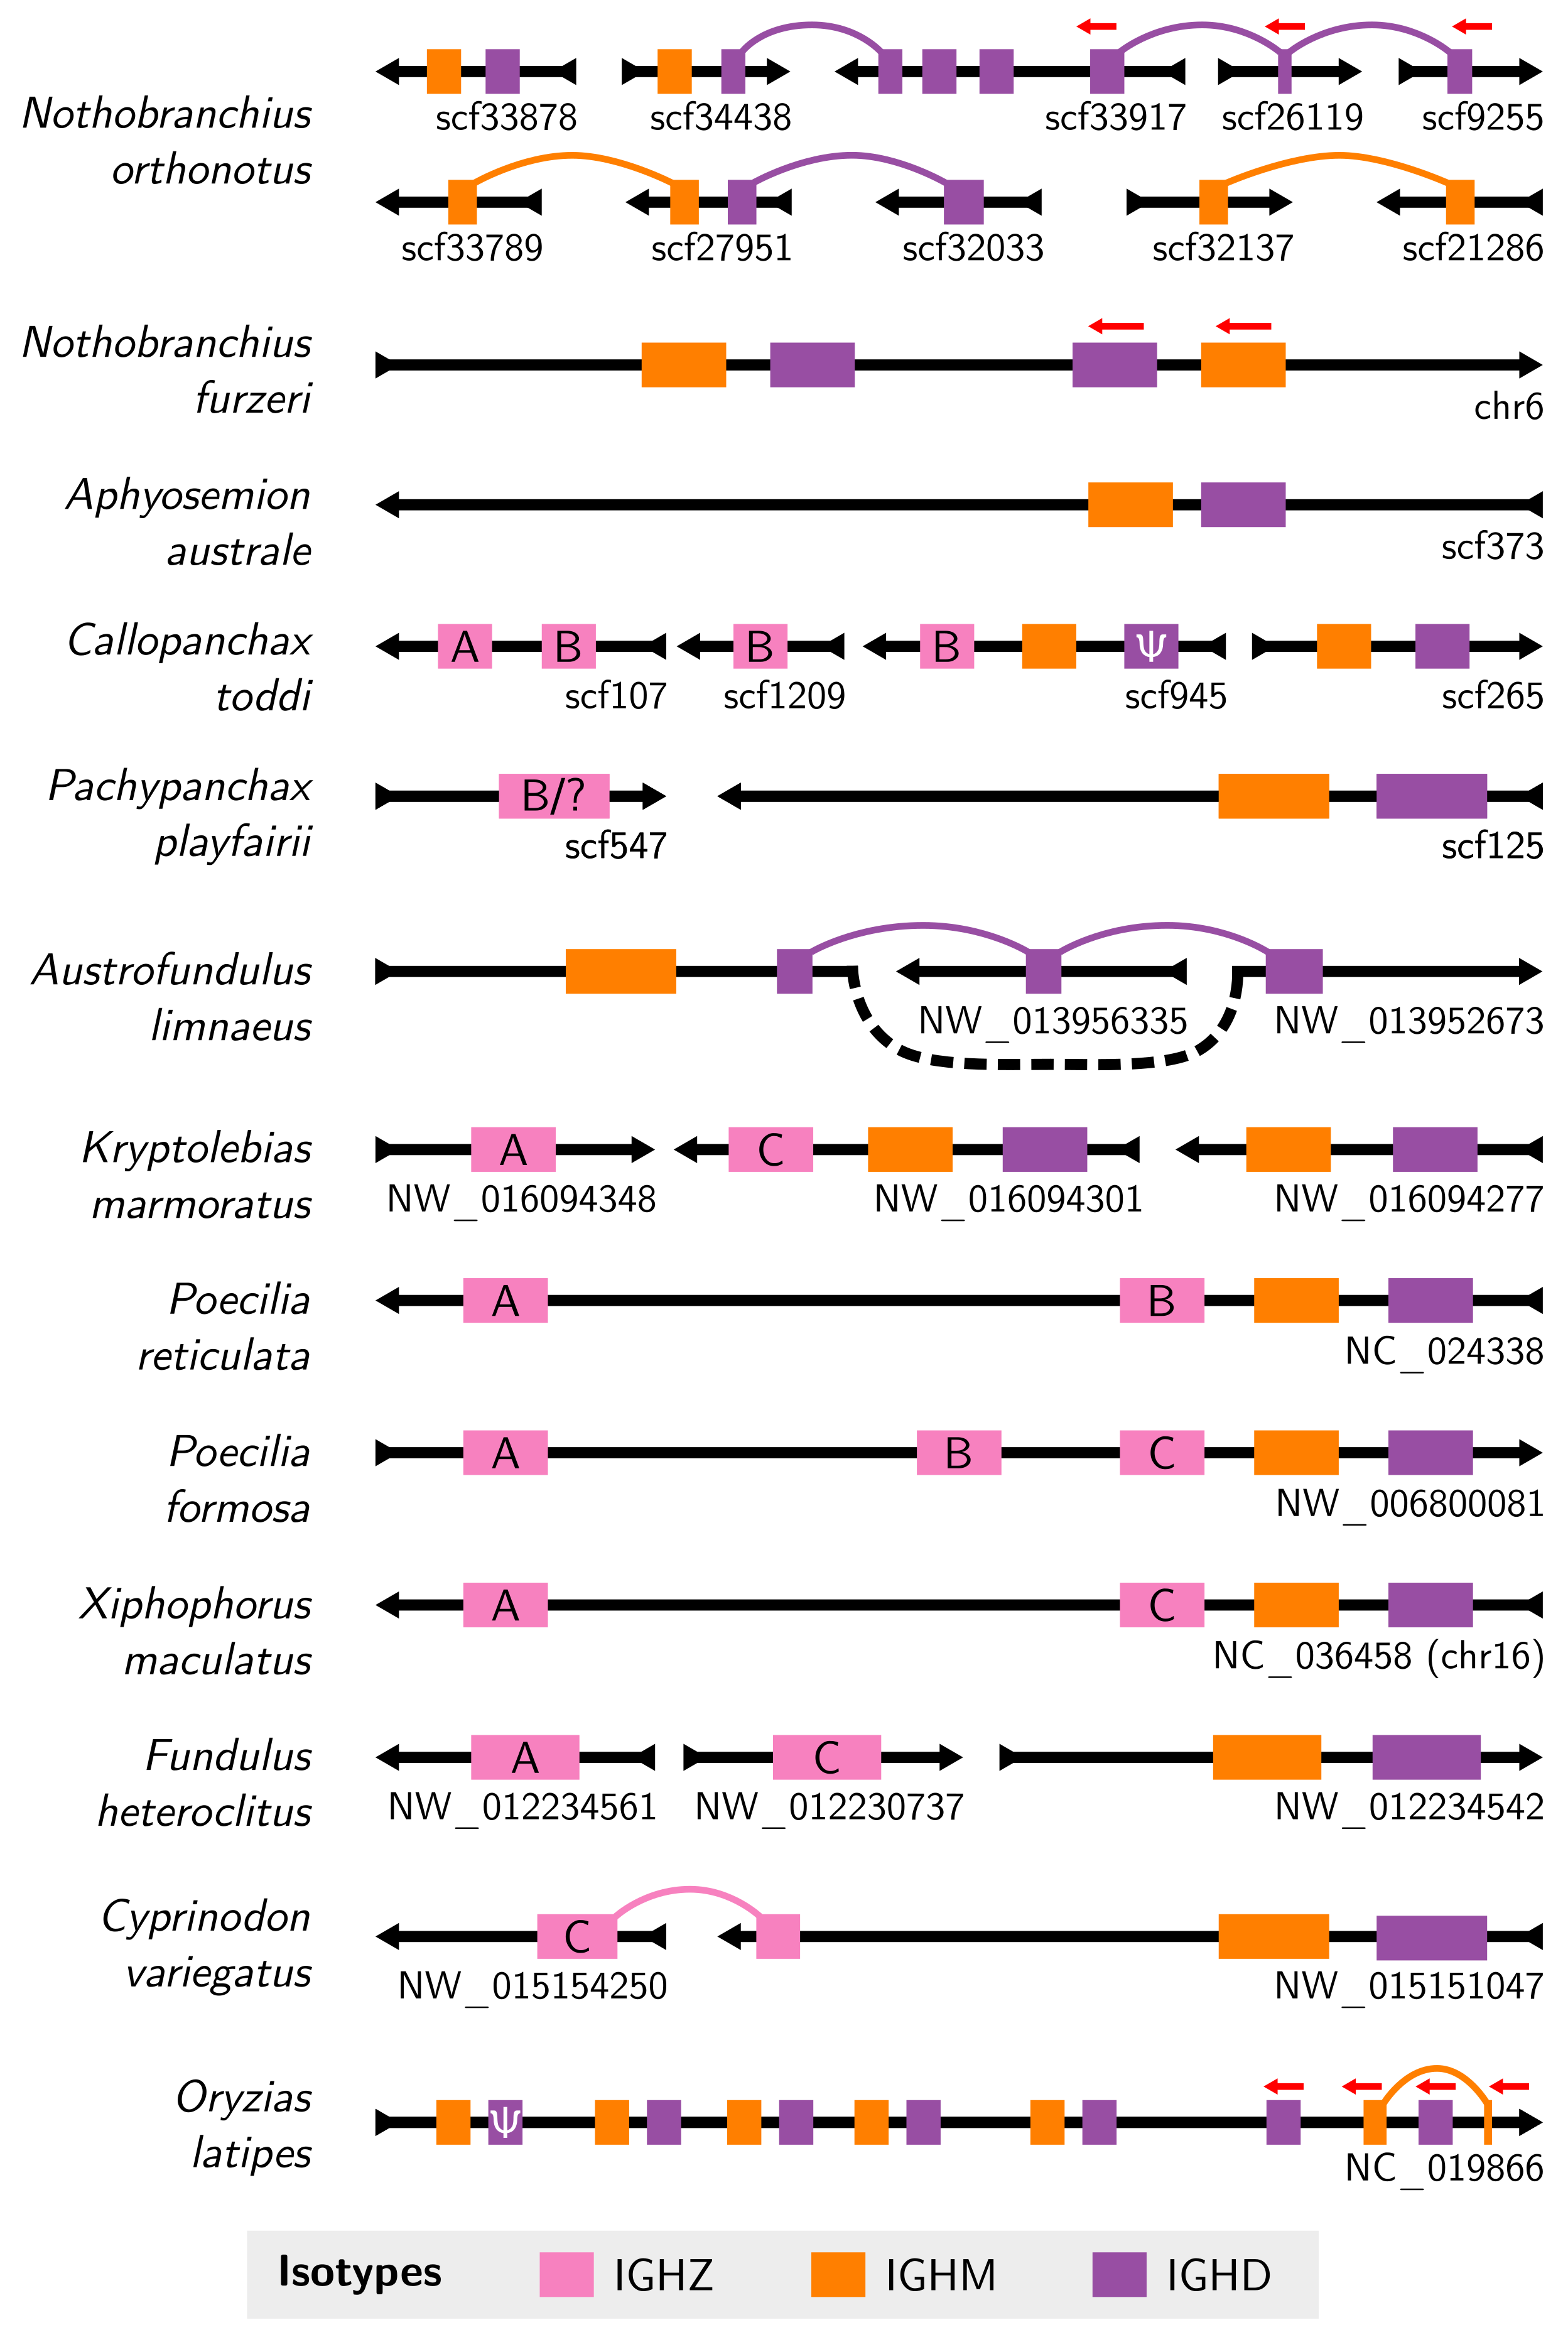
\includegraphics[width=0.9\textwidth]{_Figures/png_edited/multispecies-ch-regions}
\caption[Constant-region organisation in the Atherinomorpha]{\textbf{Constant-region organisation in the Atherinomorpha:}
Schematic of \igh{} constant regions in the genomes of thirteen species from the Atherinomorpha. Scaffold orientation is given by the black arrows; constant regions are oriented left-to-right unless otherwise specified (red arrows). Links between regions on different scaffolds indicate that exons from what appears to be the same constant region are distributed across multiple scaffolds in the order indicated; the order of unlinked scaffolds is arbitrary. The isotype of each region is given by its colour; \igh{Z} regions are further annotated with their subclass (\Cref{fig:species-tree-large-ighz}). Clearly pseudogenised constant regions are indicated by $\Psi$. Isotype length, scaffold length, and scaffold position are not to scale. Variable regions and lone, isolated constant-region exons are not shown.}
\label{fig:multispecies-ch-regions}
\end{figure}

In addition to at least one \igh{M} and \igh{D} constant region, the majority of species analysed (8 out of 13) were also found to possess at least one complete \igh{Z} constant region; of the exceptions, \species{A.}{limnaeus} exhibits an orphaned, pseudogenised \igh{Z-TM1} exon but no \cz exons in the current assembly (\Cref{fig:multispecies-ch-regions}, \Cref{tab:multispecies-ch-regions-2}), while \species{O.}{latipes}, \species{A.}{australe}, \Nfu and \species{N.}{orthonotus} display no \igh{Z} exons at all. Multiple duplications of \igh{Z} appeared even more common than for the other isotypes, with an average of 2.125 regions per \igh{Z}-bearing locus. Annotating the tree from \Cref{fig:species-tree-large-taxa} with the \igh{Z} status of each species (\Cref{fig:species-tree-large-ighz}) confirms that the loss of \igh{Z} in turquoise killifish (and related species) and medaka represent two distinct deletion events, with \textit{Austrofundulus limnaeus} potentially representing a third independent loss of \igh{Z} within the Atherinomorpha.

\begin{figure}
\centering
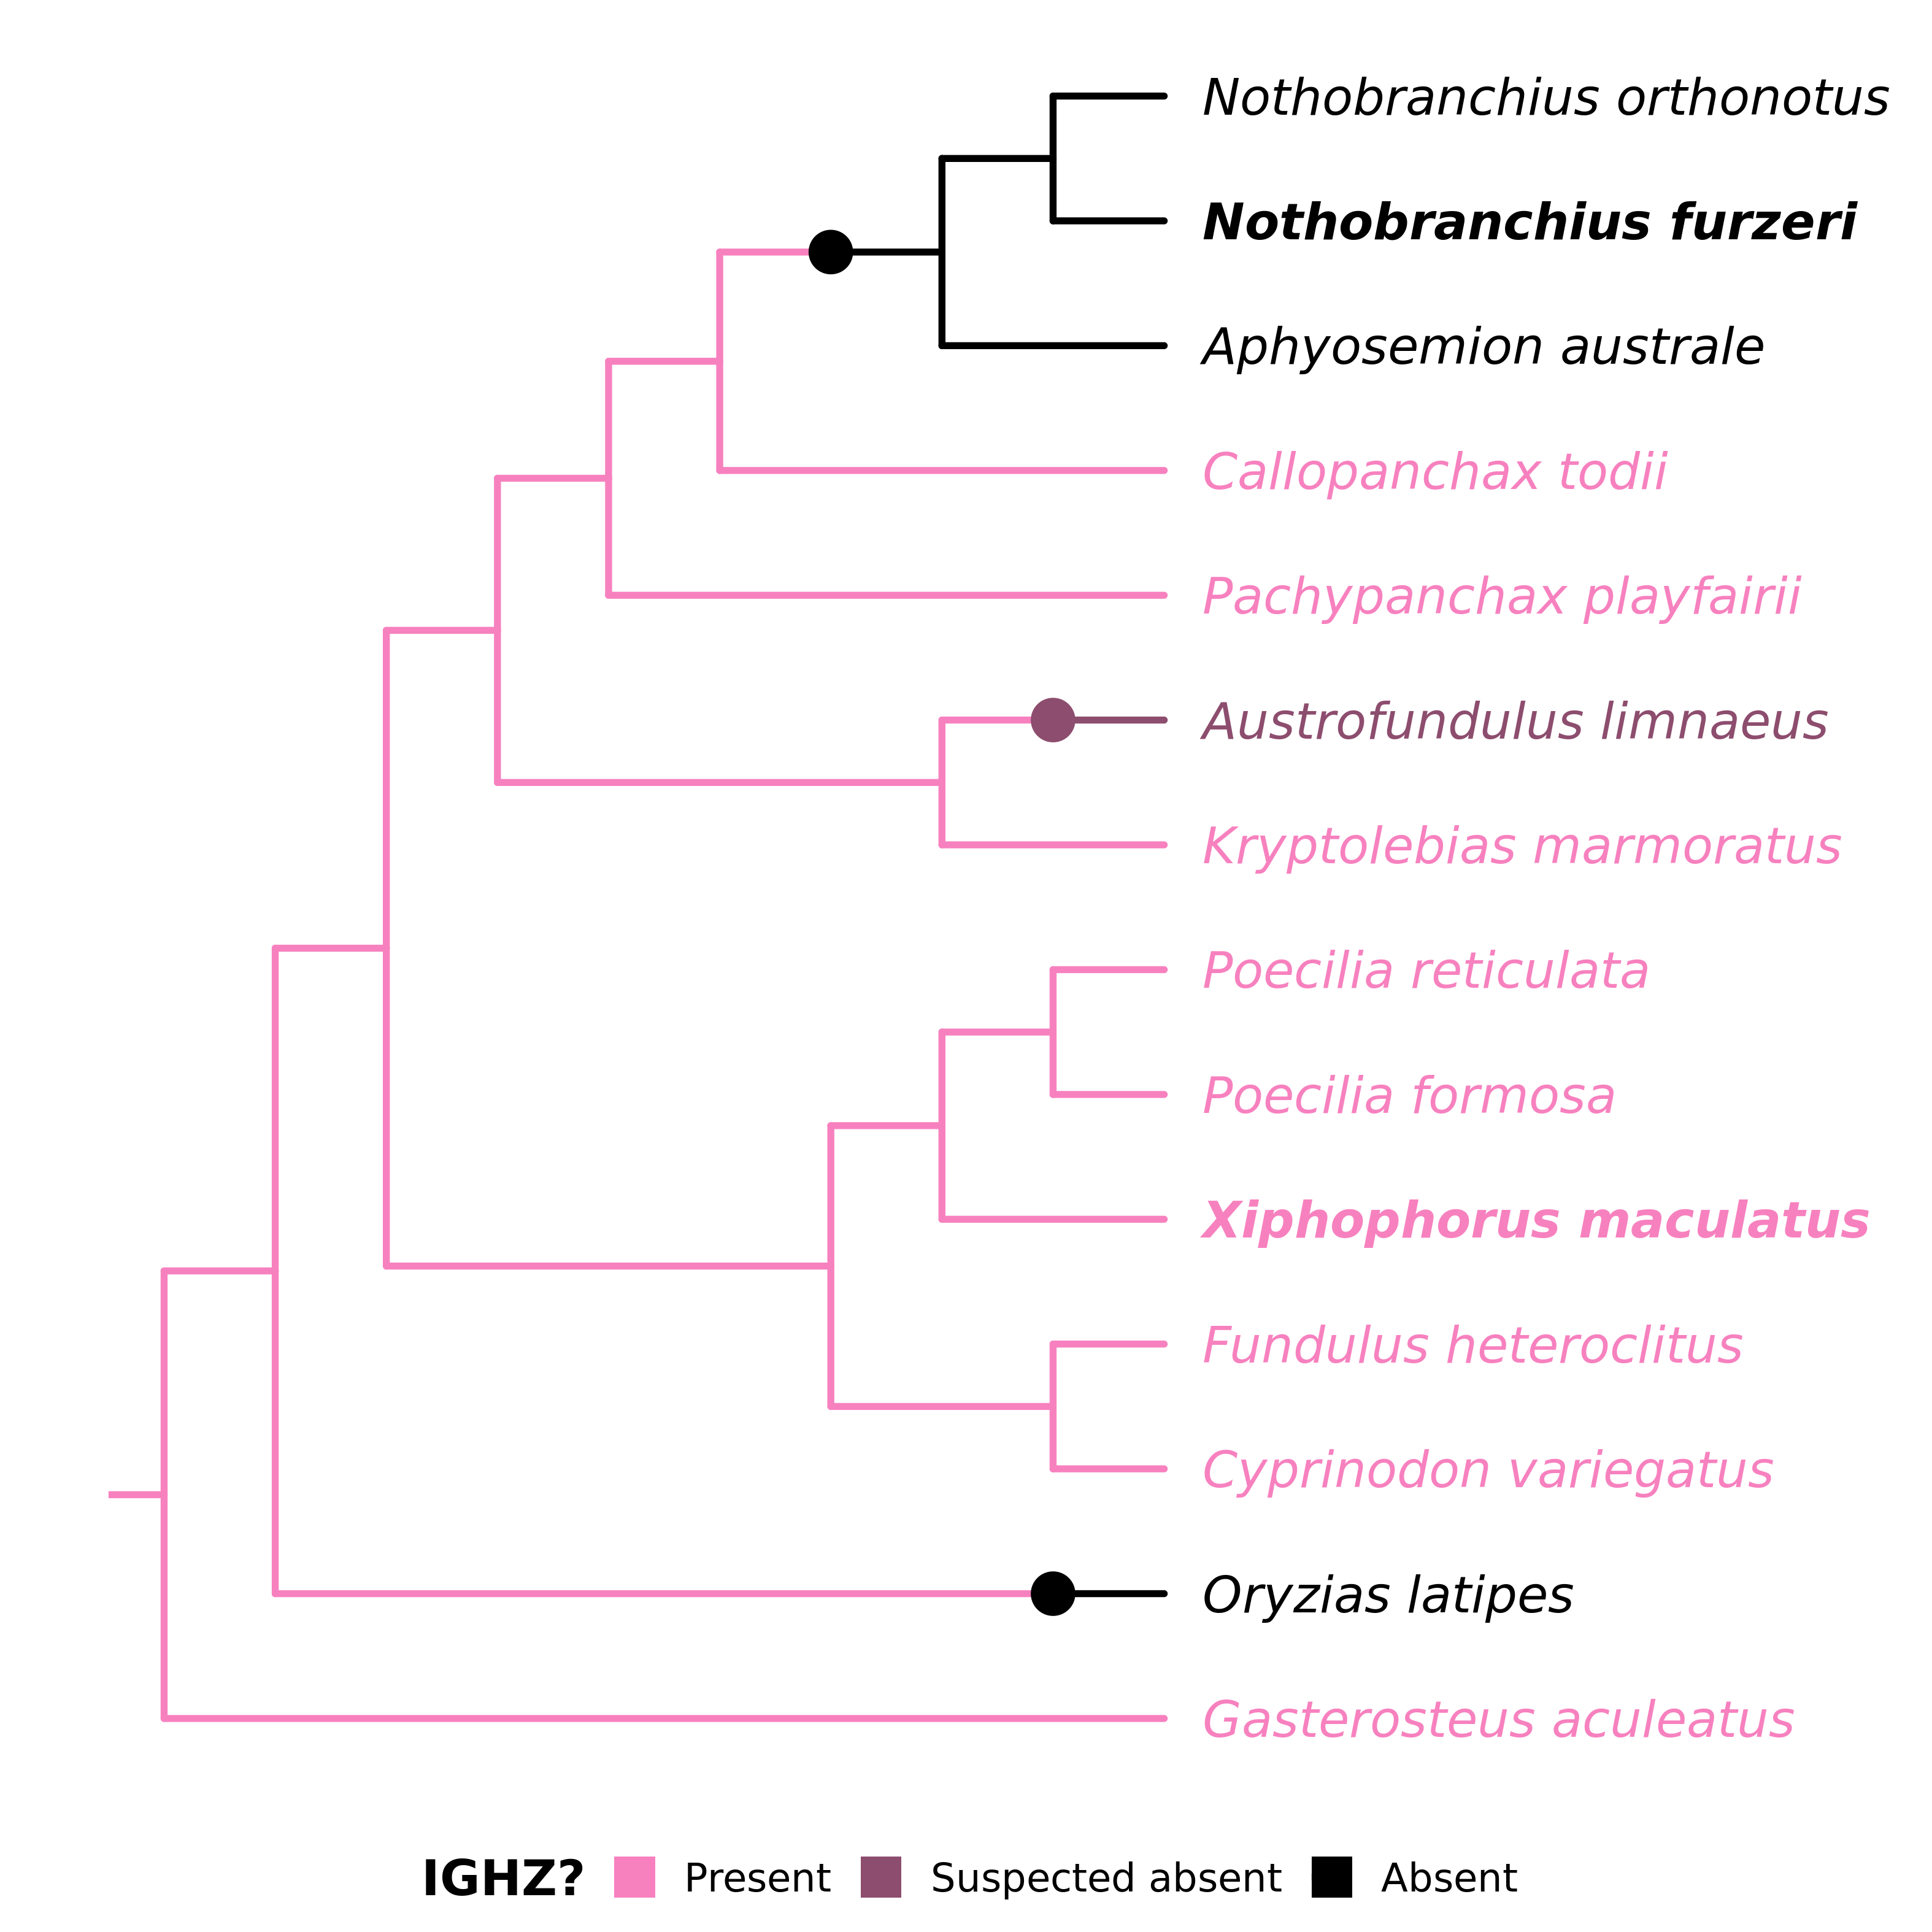
\includegraphics[width=0.9\textwidth]{_Figures/png/species-tree-large-ighz}
\caption[\igh{Z} in the Atherinomorpha has been lost multiple times independently]{\textbf{\igh{Z} in the Atherinomorpha has been lost multiple times independently:} Cladogram of species reproduced from \Cref{fig:species-tree-large-taxa}, annotated according to the known (tip nodes) or inferred (internal nodes) presence or absence of intact \igh{Z} constant regions in each species. Large coloured points on the cladogram denote sites of hypothesised state changes; \igh{Z} is assumed to be primitively present in the clade and losses to be irreversible. The currently-available genome assembly of \textit{A. limnaeus} (dark pink) contains one pseudogenised \igh{Z-TM1} exon and no \cz{} exons.}
\label{fig:species-tree-large-ighz}
\end{figure}

Apart from its repeated loss within the lineage, a second striking feature of \igh{Z} within the Atherinomorpha is its frequent presence in multiple copies per \igh{} locus; on average (geometric mean), the species analysed have approximately 1.62 \igh{Z} constant regions per \igh{M} constant region, and the same ratio veforrsus \igh{D}, suggesting a more complex evolutionary history than can be captured by a simple presence/absence metric. Concordantly, phylogenetic analysis (\Cref{fig:multispecies-cz-tree}, tree built using \program{PRANK} and \program{RAxML} on of \cz{1}--\cz{4} exon sequences) reveals three distinct lineages (or \textit{subclasses}) of \igh{Z} constant regions in the Cyprinidontiformes, each of which is present in multiple different species and appears to have been present in the common ancestor of the eight \igh{Z}-bearing species analysed (\Cref{fig:multispecies-cz-subclasses}).

\begin{figure}
	\centering
	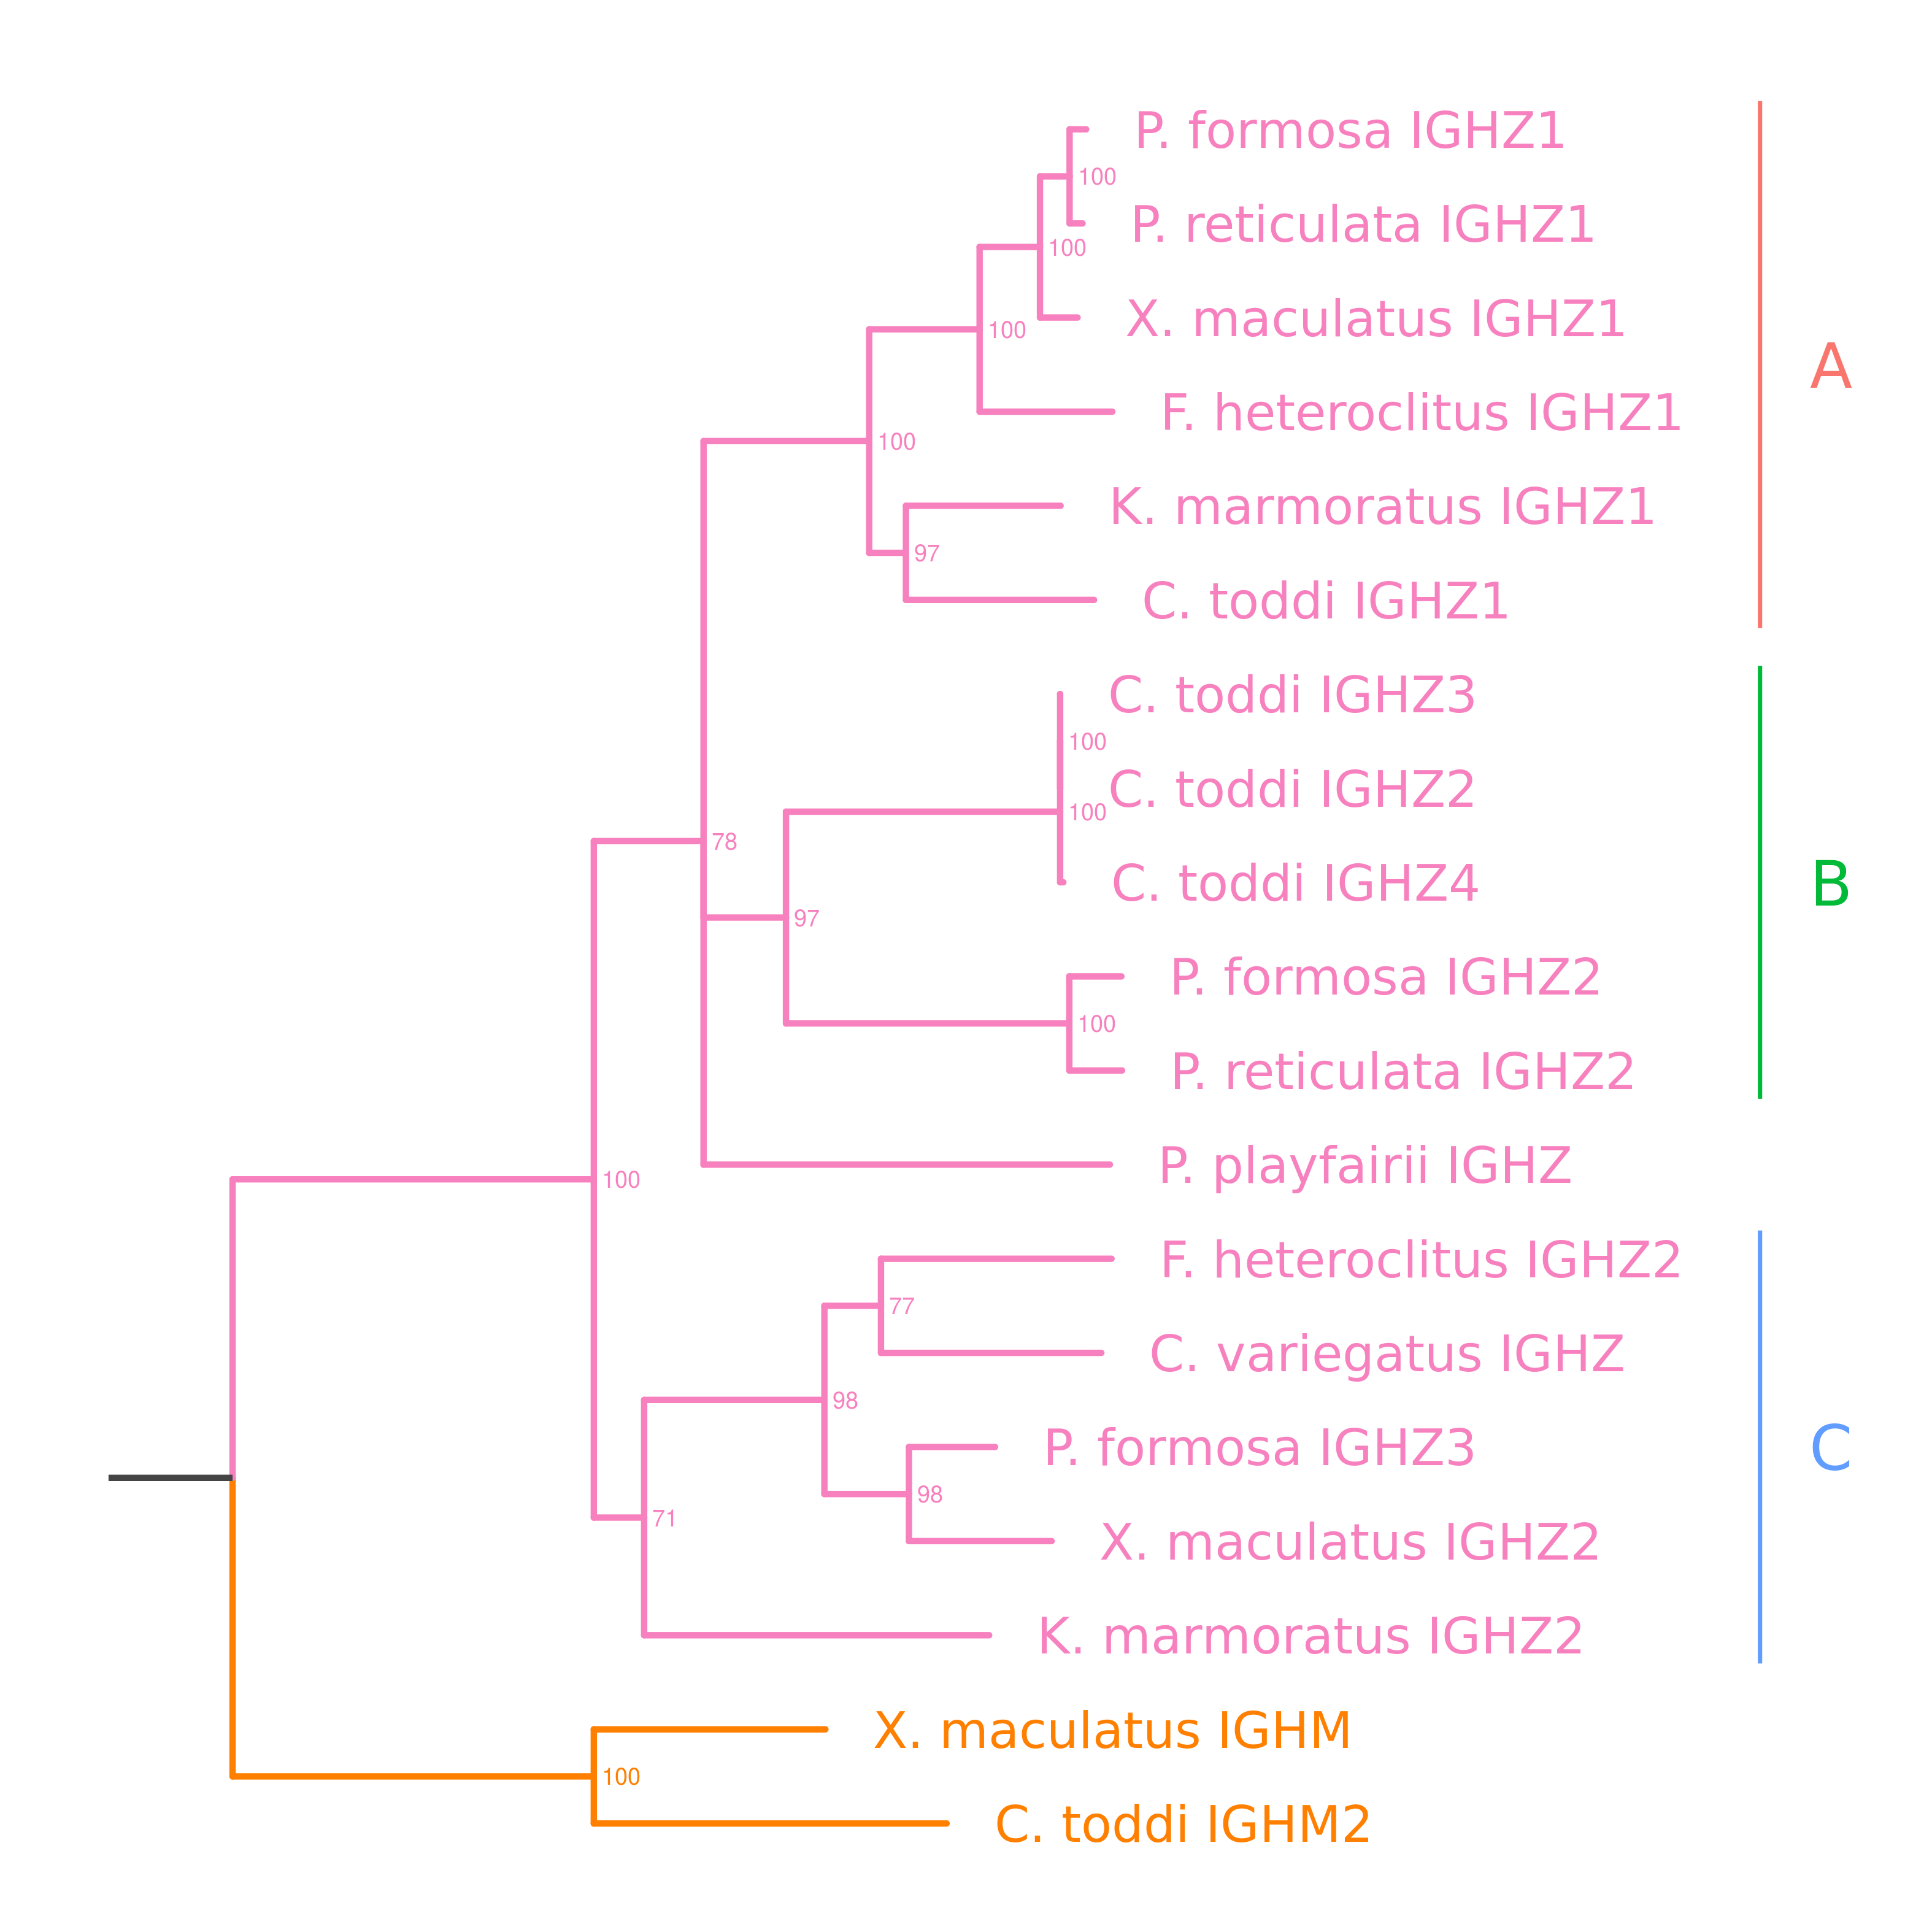
\includegraphics[width=0.9\textwidth]{_Figures/png/multispecies-cz-tree}
	\caption[\igh{Z} constant regions constitute three distinct subclasses]{\textbf{\igh{Z} constant regions constitute three distinct subclasses:} 
	Phylogram of concatenated \cz{1}--\cz{4} nucleotide sequences from \igh{Z}-bearing species in \Cref{tab:cyprinodontiform-genomes}, with \cm{1}--\cm{4} sequences from two species as an outgroup (in orange). Major clades (A--C) are annotated on the right. Support values indicate the result of rapid bootstrapping by \program{RAxML} across 1000 replicates.}
	\label{fig:multispecies-cz-tree}
\end{figure}

\begin{figure}
\centering
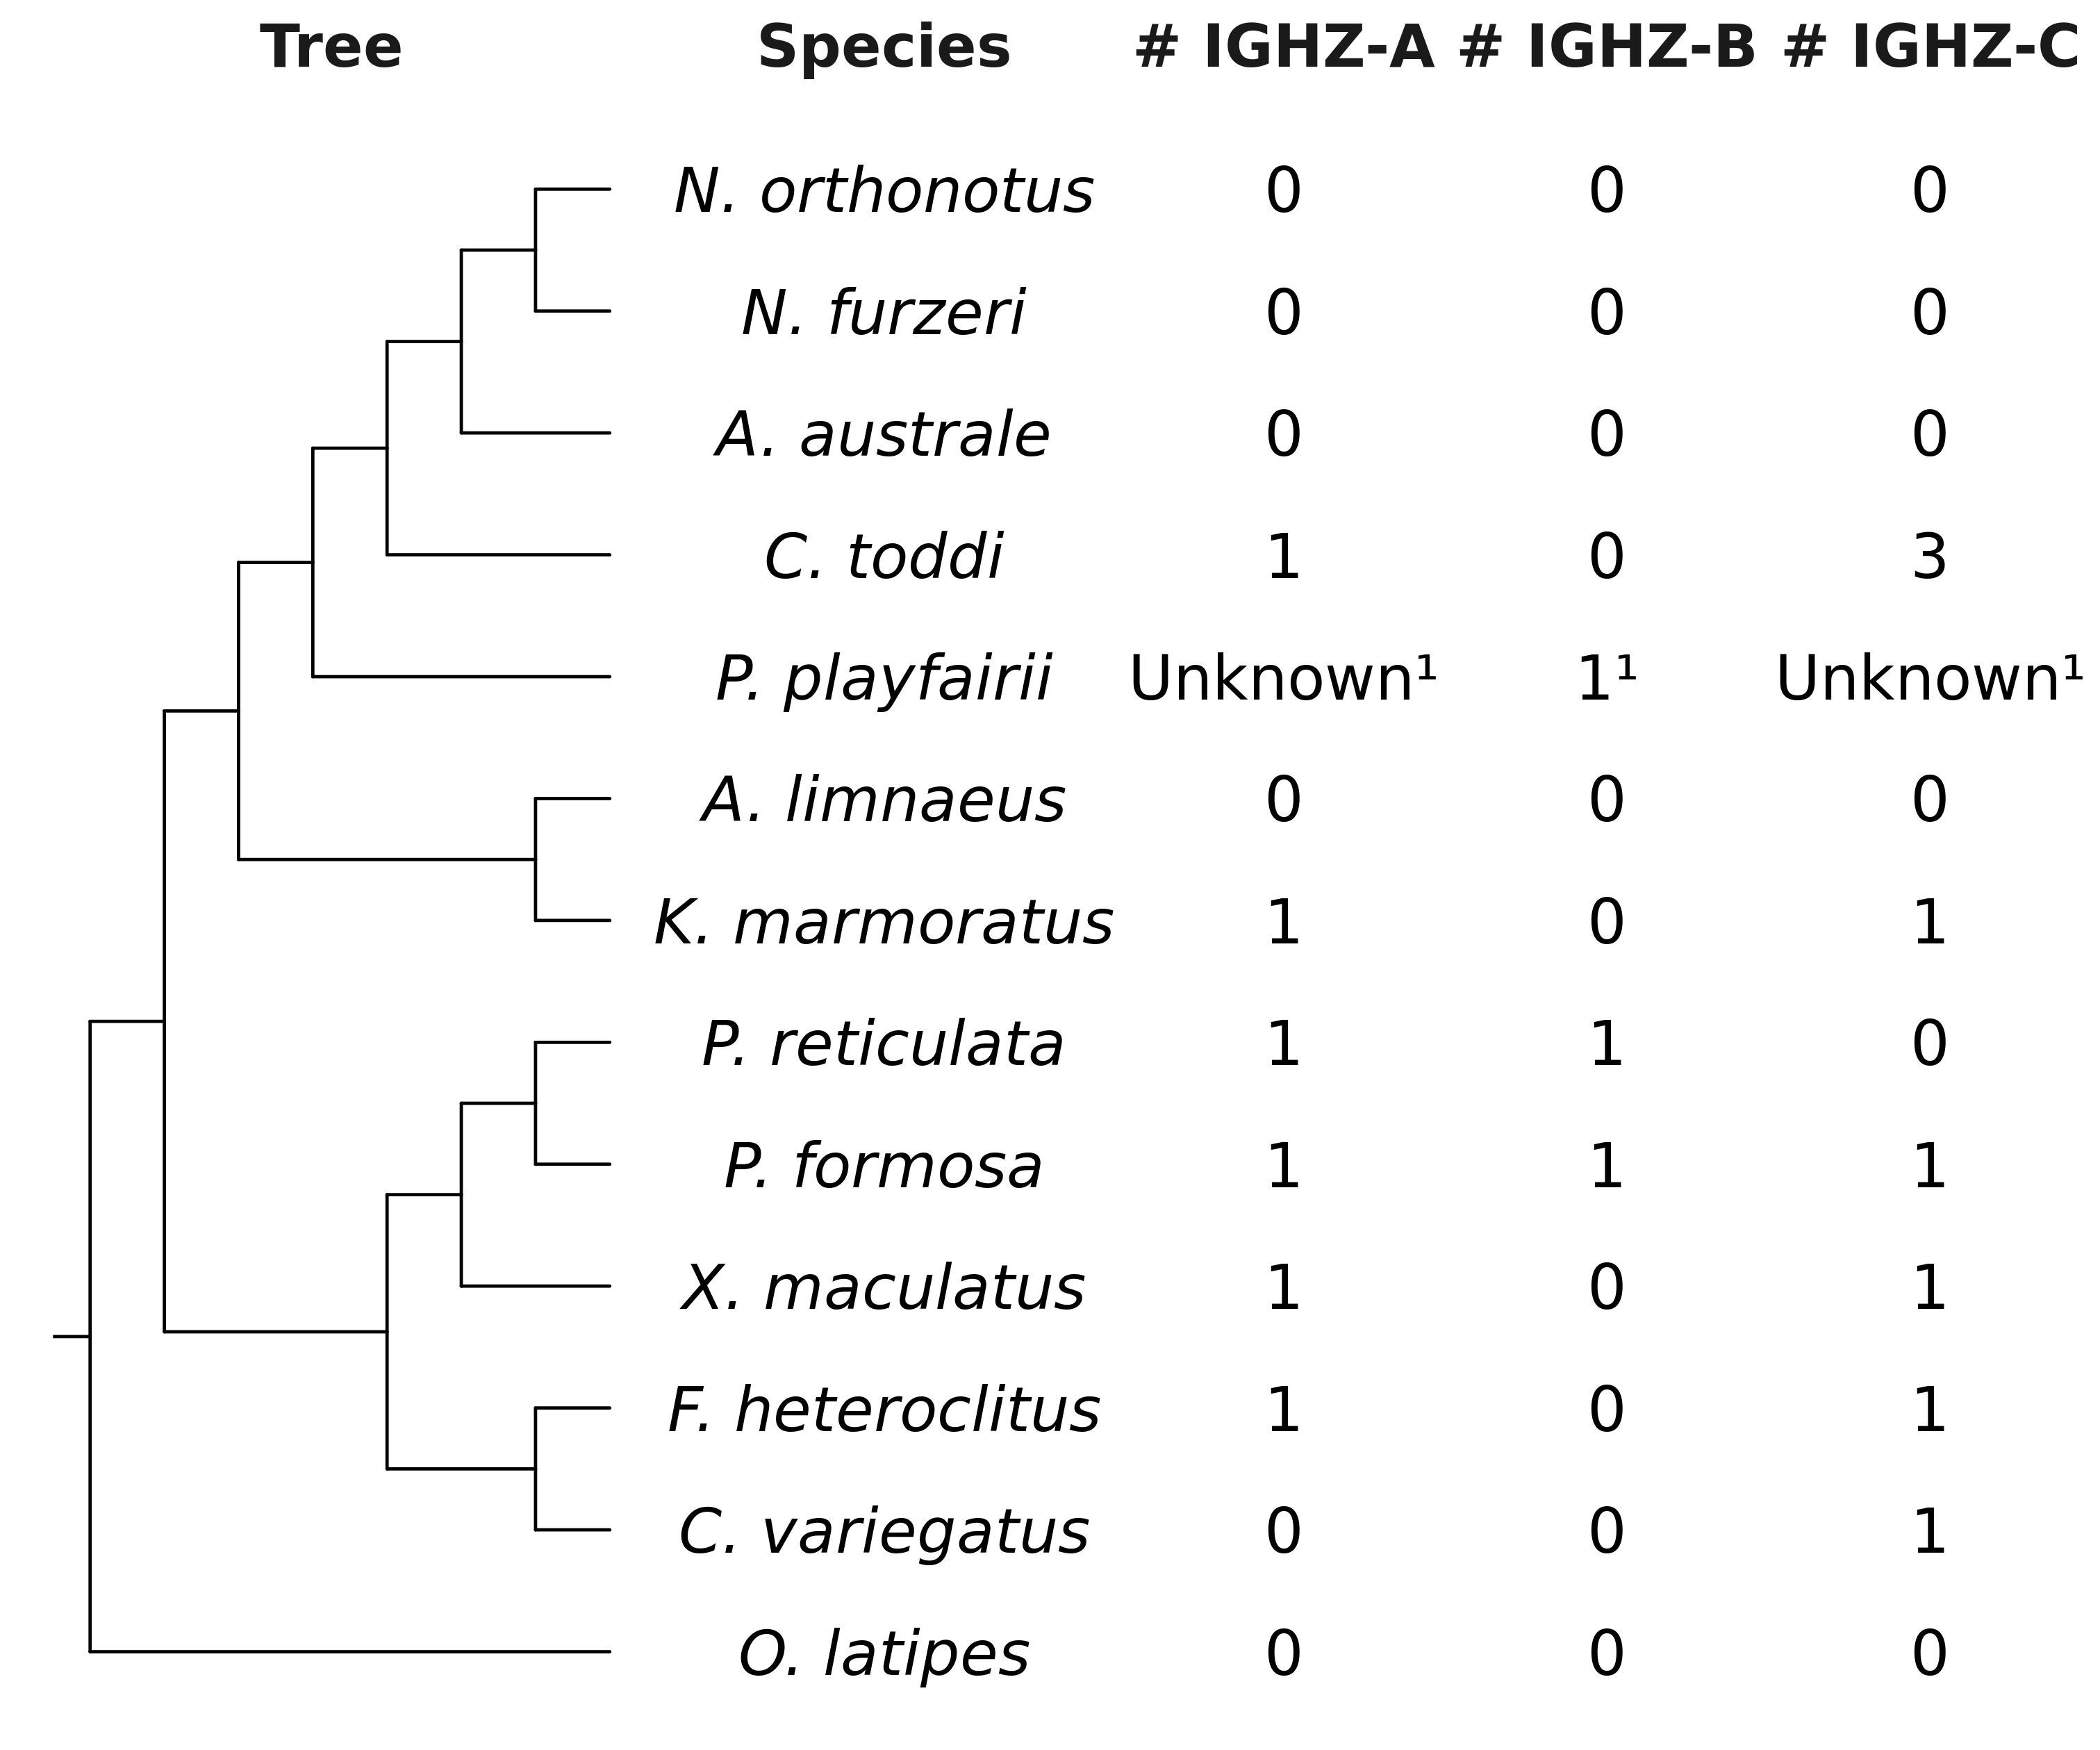
\includegraphics[width=0.8\textwidth]{_Figures/png/multispecies-cz-subclasses}
\begin{minipage}{0.7\textwidth}
\footnotesize
\begin{threeparttable}
\begin{tablenotes}
\item[1] \textit{P. playfairii} \igh{Z} \cz{1}--\cz{2} appear to be derived from \igh{Z-B}, while the other exons are of uncertain subclass origin (\Cref{fig:ppl-cz-aln}).
\end{tablenotes}
\end{threeparttable}
\end{minipage}
\caption[\igh{Z} subclasses in the Atherinomorpha]{\textbf{\igh{Z} subclasses in the Atherinomorpha:} Cladogram of atherinomorph species with characterised \igh{Z} constant regions, annotated with the number of regions belonging to each \igh{Z} isotype in each species. All three subclasses are present in at least one species in both major branches of the cyprinodontiform clade, suggesting that they were all present in the common ancestor of this grouping.}
\label{fig:multispecies-cz-subclasses}
\end{figure}


Only one \igh{Z} constant region from the analysed species could not be confidently assigned to one of these three subclasses, namely the single \igh{Z} of \species{Pachypanchax}{playfairii} (\Cref{fig:multispecies-cz-tree}). In order to more closely investigate the relationships of \igh{Z} in this species, the exon sequences of \species{P.}{playfairii} \cz{1}--\cz{4} were separately aligned to the \cz{} exons of all other \igh{Z}-bearing species using Needleman-Wunsch global alignments, and the distribution of alignment scores was plotted in \Cref{fig:ppl-cz-aln}
. The results show a striking difference in alignment behaviour between the exons, with \cz{1} and \cz{2} aligning much more strongly to exons from the B subclass and \cz{3} and \cz{4} showing more ambiguous affinity for either A- or C-subclass sequences. This unexpected behaviour indicates that the \species{P.}{playfairii} \igh{Z} sequence is the result of a deletion or fusion event combining the first two exons of a B-lineage \igh{Z} constant region with the latter exons of a constant region from another lineage, resulting in a chimeric gene with ambiguous ancestry.

\begin{figure}
	\centering
	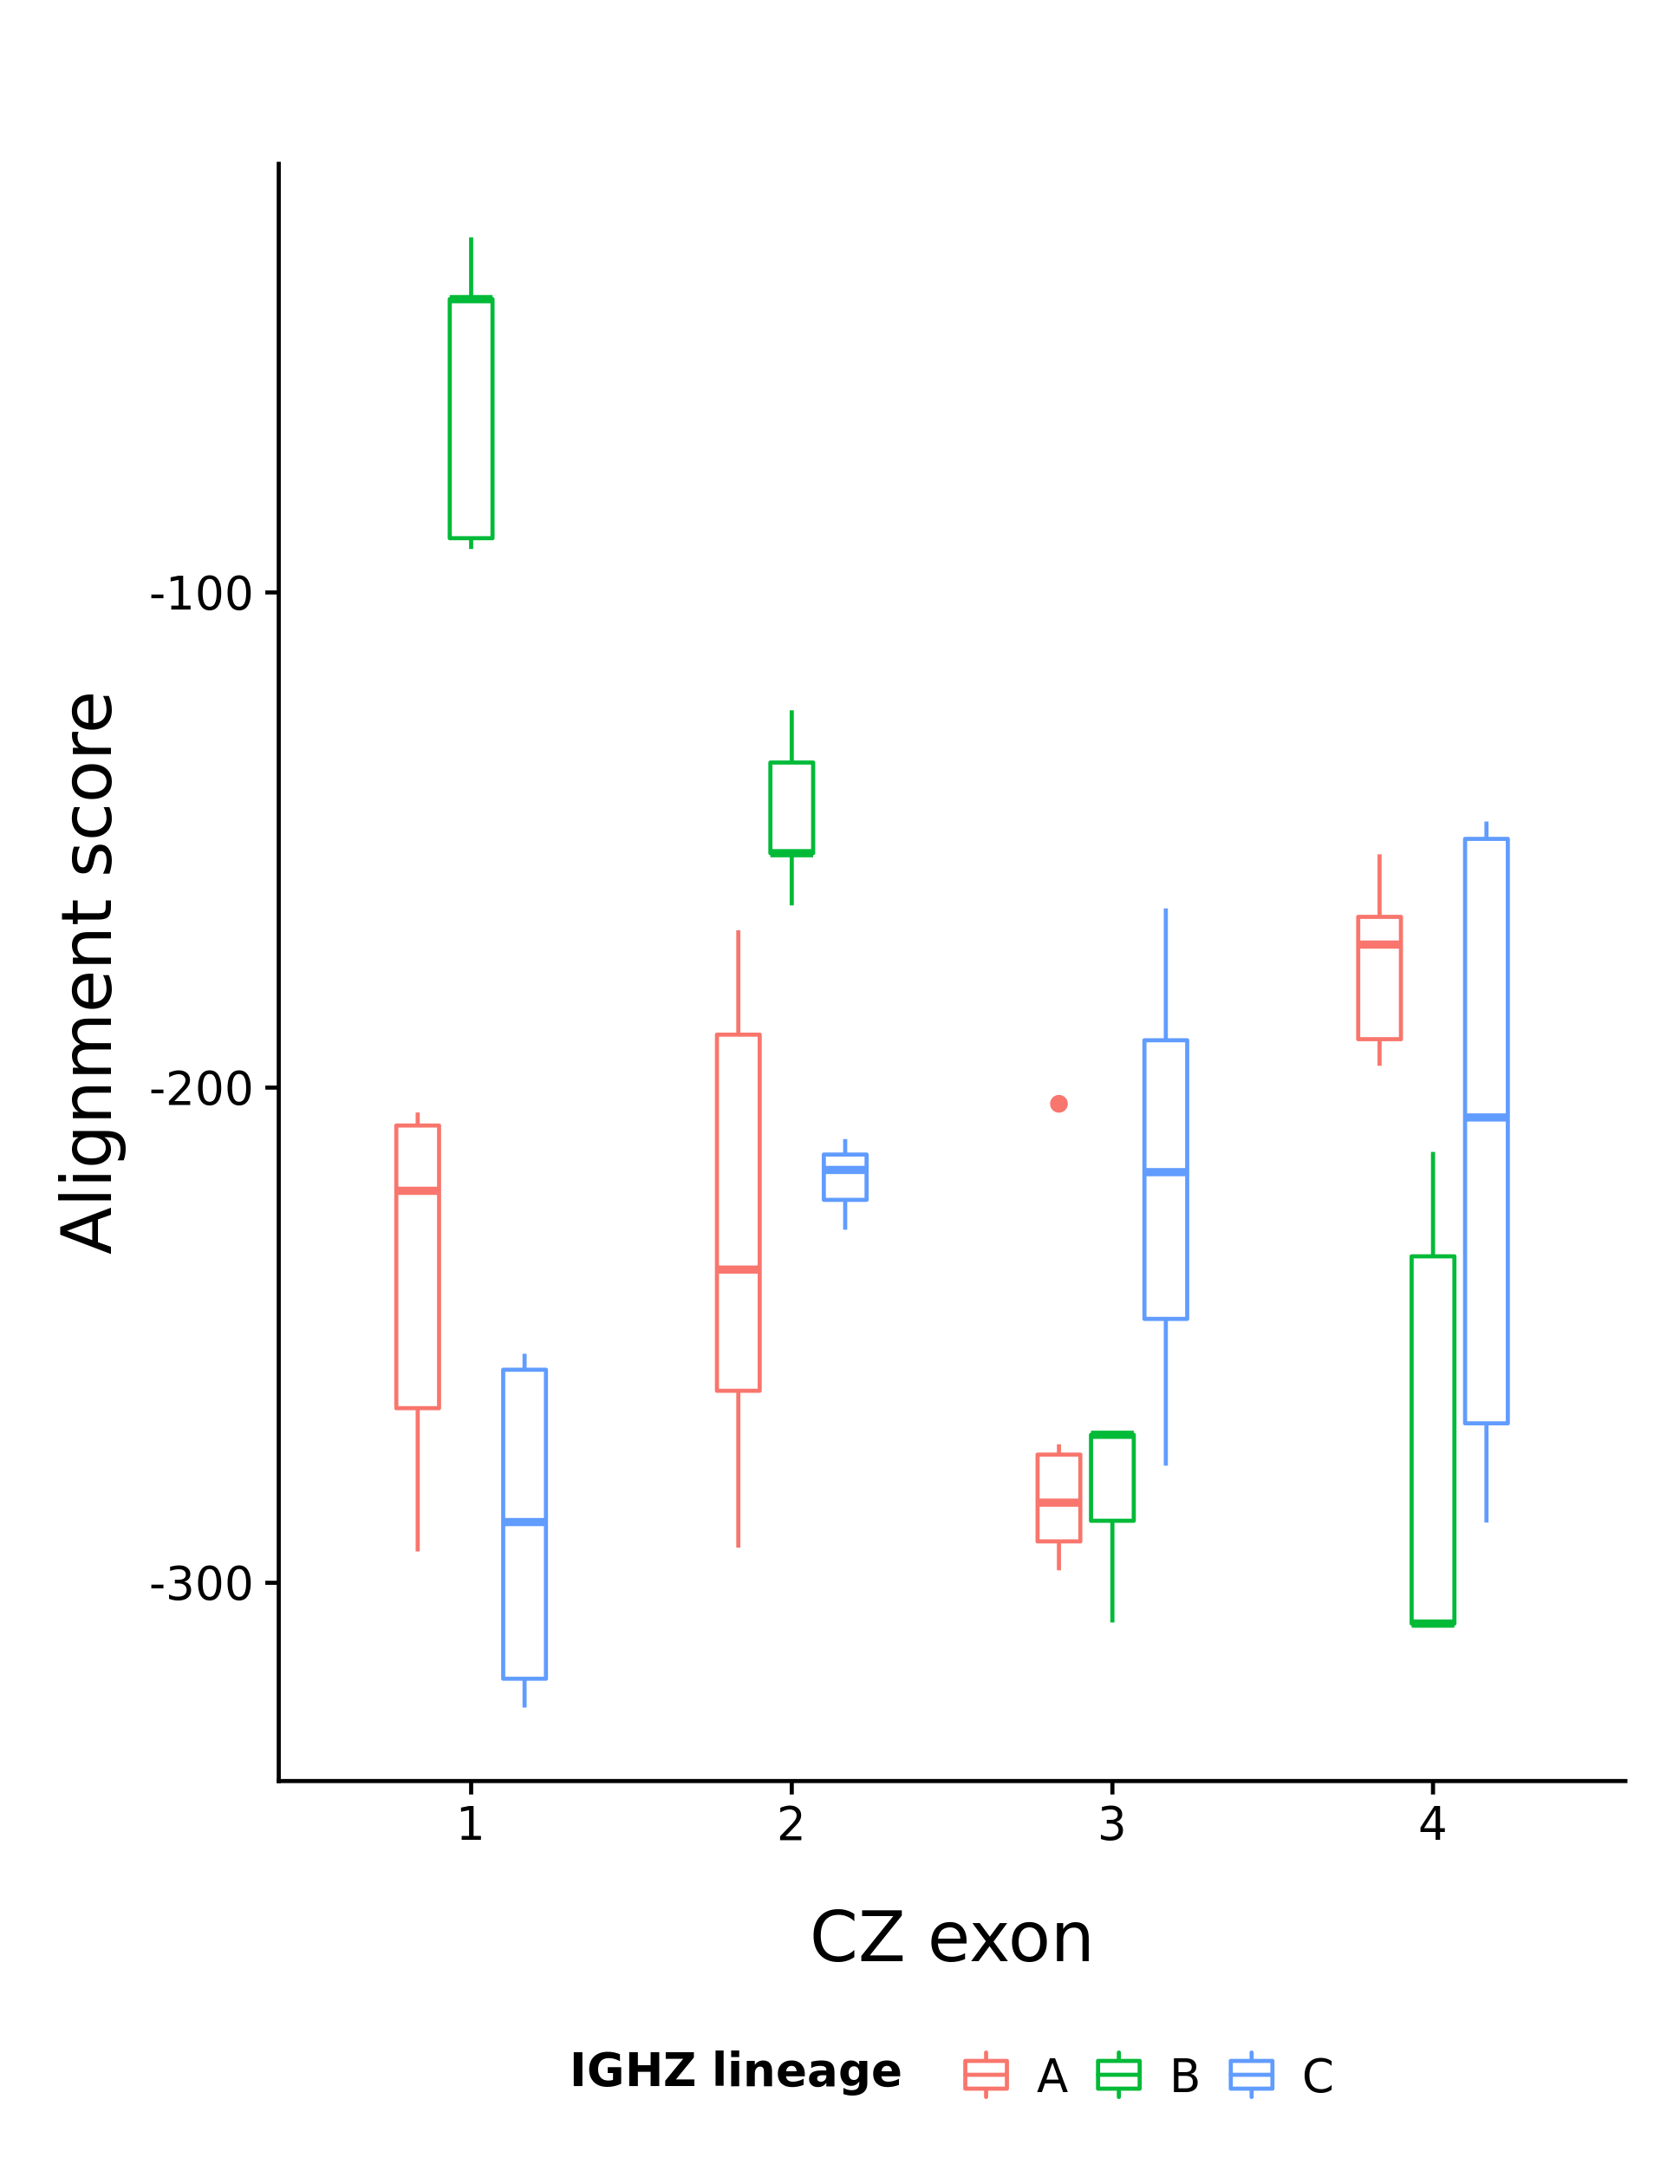
\includegraphics[width=0.7\textwidth]{_Figures/png/ppl-cz-aln-aa.png}
	\caption[Subclass affinity of \species{Pachypanchax}{playfairii} \igh{Z}]{\textbf{Subclass affinity of \species{Pachypanchax}{playfairii} \igh{Z}:} 
	Boxplots of Needleman-Wunsch alignment scores between the amino-acid sequences of \species{P.}{playfairii} \cz{} exons and those of seven other \igh{Z}-bearing cyprinodontiform species, demonstrating the differing affinity of diferent \species{P.}{playfairii} exons for each of the three \igh{Z} subclasses.}
	\label{fig:ppl-cz-aln}
\end{figure}
	
In summary, in addition to the still-universal primitive antibody classes \igh{M} and \igh{D}, the cyprinodontiforms ancestrally possessed both at least three variants of \igh{Z}, giving rise to multiple subclasses of \igh{Z} constant regions evolving in parallel across the clade. Each of these subclasses appears to have been lost in multiple cyprinodontiform species, with different species showing distinct patterns of retention and loss, and in at least one lineage -- that of \species{Pachypanchax}{playfairii} -- two different \igh{Z} lineages have fused to produce a chimeric isotype. All three subclasses are missing from a subset of species in the Nothobranchiidae (including \nfu), and also appear to have been independently lost in \species{Austrofundulus}{limnaeus}. Taken together, these data suggest a high degree of complexity and volatility in the evolution of mucosal adaptive immunity in the Cyprinodontiformes.


	% Discussion

	%	The examination of the constant-region structures present in the \Xma IGH locus therefore reveals three notable features that differ in state between medaka, turquoise killifish, and the southern platyfish. Most strikingly, the absence of IGHM in medaka and killifish, but its presence in platyfish, strongly suggests that the isoform has been lost independently in the two groups. Conversely, the presence of a four-exon IGHM-TM in medaka and killifish, but a five-exon configuration in platyfish, is less clear-cut: it may indicate an independent change in medaka and killifish that is absent in platyfish, but may also plausibly represent a reversion in platyfish to the more-primitive five-exon state. Without a deeper understanding of the currently-unknown physical underpinnings of this observed difference in splicing behaviour, this question can only be addressed through analysis of RNA-seq data from a large number of related species, something beyond the scope of the present investigation. % TODO: Do it anyway?
%	Finally, the presence of a (\cd{2}-\cd{3}-\cd{4}) duplication in both platyfish and killifish, but not in medaka, suggests that this may be a shared primitive feature of the Cyprinodontiforms; however, given the apparent recurrence of this duplication pattern in many different groups across the teleosts, a strong conclusion cannot be drawn without a higher-resolution phylogenetic analysis of a larger number of related species.
% TODO: Move to multispecies section intro

	%	TODO: Move to multilocus section. Alongside this, I performed a more limited characterisation of the \textit{IgH} constant regions in 9 %?
%	additional cyprinodontiform and beloniform species, to assess the broader patterns of immunoglobulin heavy chain evolution within these groups (\Cref{sec:comparative-loci}). The results of these additional investigations repeatedly called into question the hypothesis of homology in IgH locus ideosyncracies between medaka and turquoise killifish, and suggest a model of rapid locus evolution within this diverse and important teleost clade.
	
	% TODO: Move to discussion section.
	% TODO: Relationship between killifish Vs and other species
	% TODO: Evolution of IGH1 vs 2
	% TODO: Discussion of mucosal immunity in absence of IGZ
		% TODO: Discuss smallness of killifish locus in the context of relaxed purifying selection and short life span
	% TODO: Section on "Investigating the evolutionary relationship between IGH1 and IGH2"
	% Keep for discussion:
%\q{Given the lack of IgZ in this species, how do you think they carry out mucosal immunity?}
%
%I'd assume using IgM. It's the primitive antibody and is expressed in secreted form in the killifish gut. I haven't investigated the protein expression so it's hard to say for sure, but I'd guess that's the answer. It's also quite possible, lacking a specialised mucosal class, that the answer is ``not very well". It would be very interesting to compare mucosal immune function in species with and without IgZ, especially if those species are closely related.
%
%Given the impressive results indicating the specificity of IgT for mucosal immunity in trout, and the lack of mucosal response of IgM in that species, it would be very interesting to see what mucosal responses look like in a species that lacks that isotype -- is IgM much more responsive and expressed in the gut than in IgT-possessing species, or is the mucosal response just worse?
	% (Incidentally, it would be great to see whether any B-cells in TK show recombinations in both subloci, vs one or the other. Single-cell DNA sequencing could plausibly do this.)

%	The specialised mucosal isotype \igh{Z} is present in the majority of teleost \igh{} loci characterised so far, including several species (including stickleback and fugu) relatively closely related to the Atherinomorpha; the possession of \igh{Z} therefore appears to be primitive to most groups of teleost fish. The striking absence of the isotype in both medaka and turquoise killifish (\Cref{sec:nfu-locus-constant}), the first two characterised \igh{} loci from the Atherinomorpha, suggested that the lack of \igh{Z} may have occurred in the common ancestor of both species and so be primitive both the Beloniformes and Cyprinodontiformes; however, the surprising presence of two distinct \igh{Z} loci in the locus of the southern platyfish \xma convincingly falsified this hypothesis and indicated that the loss of \igh{Z} in medaka and turquoise killifish occurred independently in their respective lineages (\Cref{sec:xma-locus-constant}). % TODO: For discussion
% It is not known whether these subclasses have distinct functional properties, or how these % TODO: For discussion








	



